\documentclass{beamer}

\usepackage{cmap}
\usepackage[english,russian]{babel} % add eng,rus(base) package
\usepackage[T1,T2A]{fontenc}        % add eng,rus encoding support
\usepackage[utf8]{inputenc}         % add UTF8 support

% Use it for English document
%\usepackage[utf8]{inputenc} % add UTF8 support
%\usepackage{fontspec}       % to use any font known to the operating system
%\setmainfont{PT Serif}      % set defolt font

\usepackage{amsmath, amsfonts, amssymb, amsthm, mathtools} % add math support

\linespread{1}               % length between str
\setlength{\parindent}{16pt} % red str
\setlength{\parskip}{6pt}   % length between paragraphs

\usepackage[backend=biber, style=authoryear-icomp]{biblatex}
\addbibresource{$HOME/latex-templates/biblio.bib}            % path to bibliography base

\usetheme{Madrid}
\setbeamertemplate{frametitle}[default][center]

\renewcommand{\thefootnote}{\arabic{footnote}}
 % here is document's settings for russian
%\input{$HOME/studyproject/universe/history/preamble-beamer-eng.tex} % here is document's settings for english


\title{Интервенция в годы гражданской войны}
\author{Немков Н.М.}
\institute[МГТУ]{МГТУ им. Н.Э. Баумана}
\date{25.03.2024}
\logo{
\includegraphics[width=1cm]{images/logo}}

\begin{document}

\begin{frame}
\maketitle
\end{frame}

\section{Введение}
\begin{frame}{Введение}
	Расспад Российской Империи дал возможность начать завоевание территоий для стран Антанты и Тройственного союза

	Беломому движению они также оказывали материальную помощь оружием и обмундированием
\end{frame}

\section{Север}
\begin{frame}{Север}
	В 1918 году был высажен Английский корпус, для занятия Мурманска и Архангельска с целью контроля путей сообщения и торговли
\end{frame}



\begin{frame}{}
	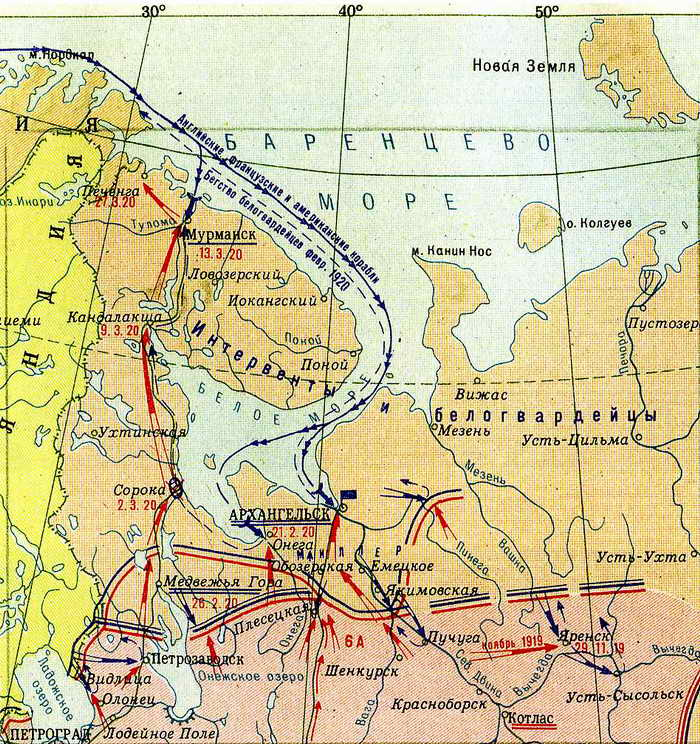
\includegraphics[width=0.8\textwidth]{images/int-north.jpg}
\end{frame}


\section{Восток}
\begin{frame}{Восток}
	Япония и США


	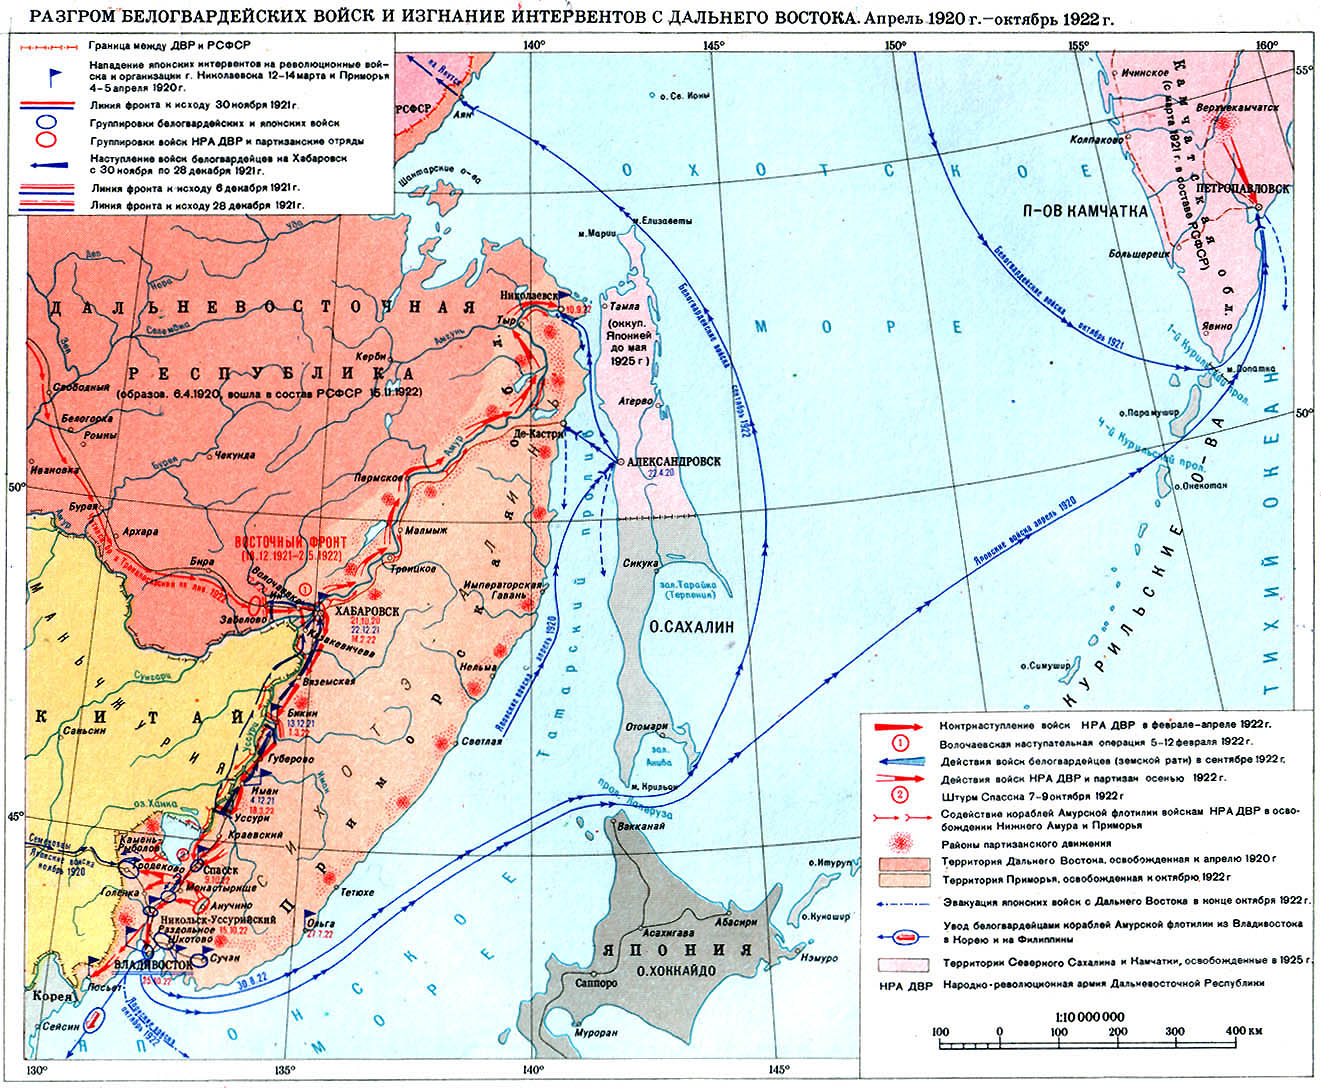
\includegraphics[width=0.7\textwidth]{images/int-east.jpg}
\end{frame}




\section{Юг}
\begin{frame}{Юг}
	Франция и Англия


	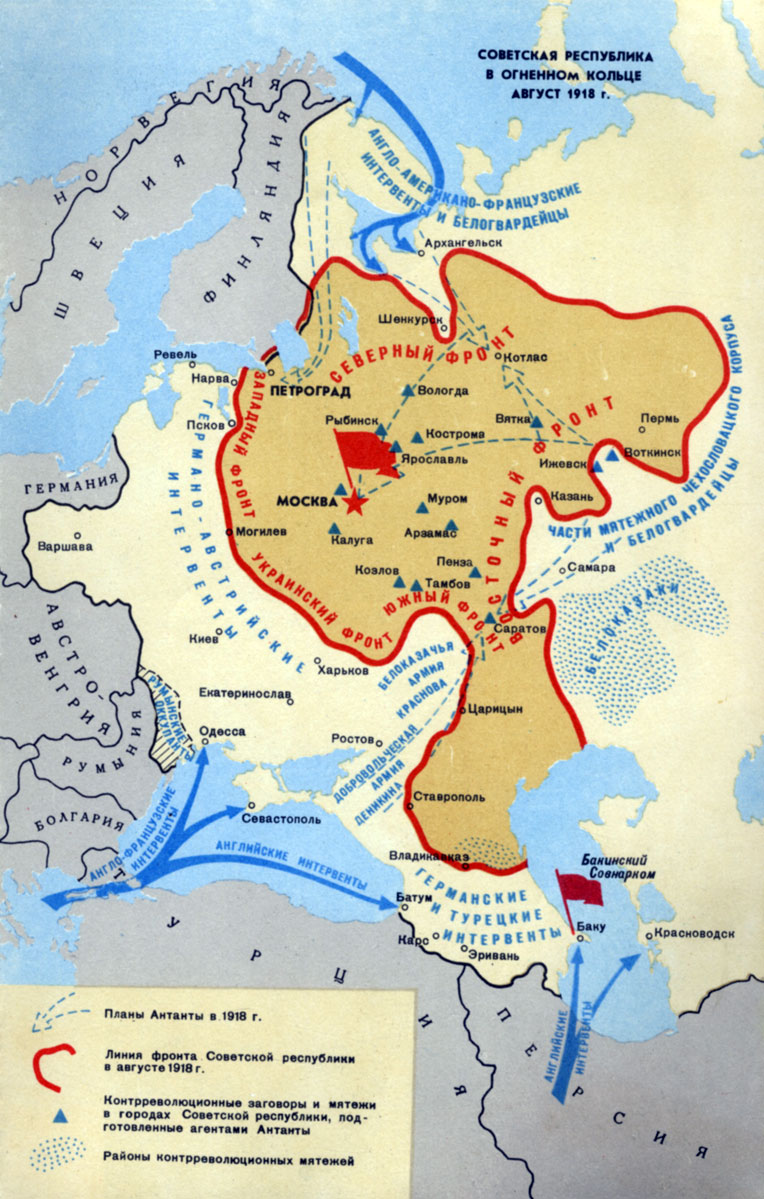
\includegraphics[width=0.5\textwidth]{images/int-south.jpg}
\end{frame}



\section{References}
\begin{frame}[t]{References}
	%\printbibliography
	%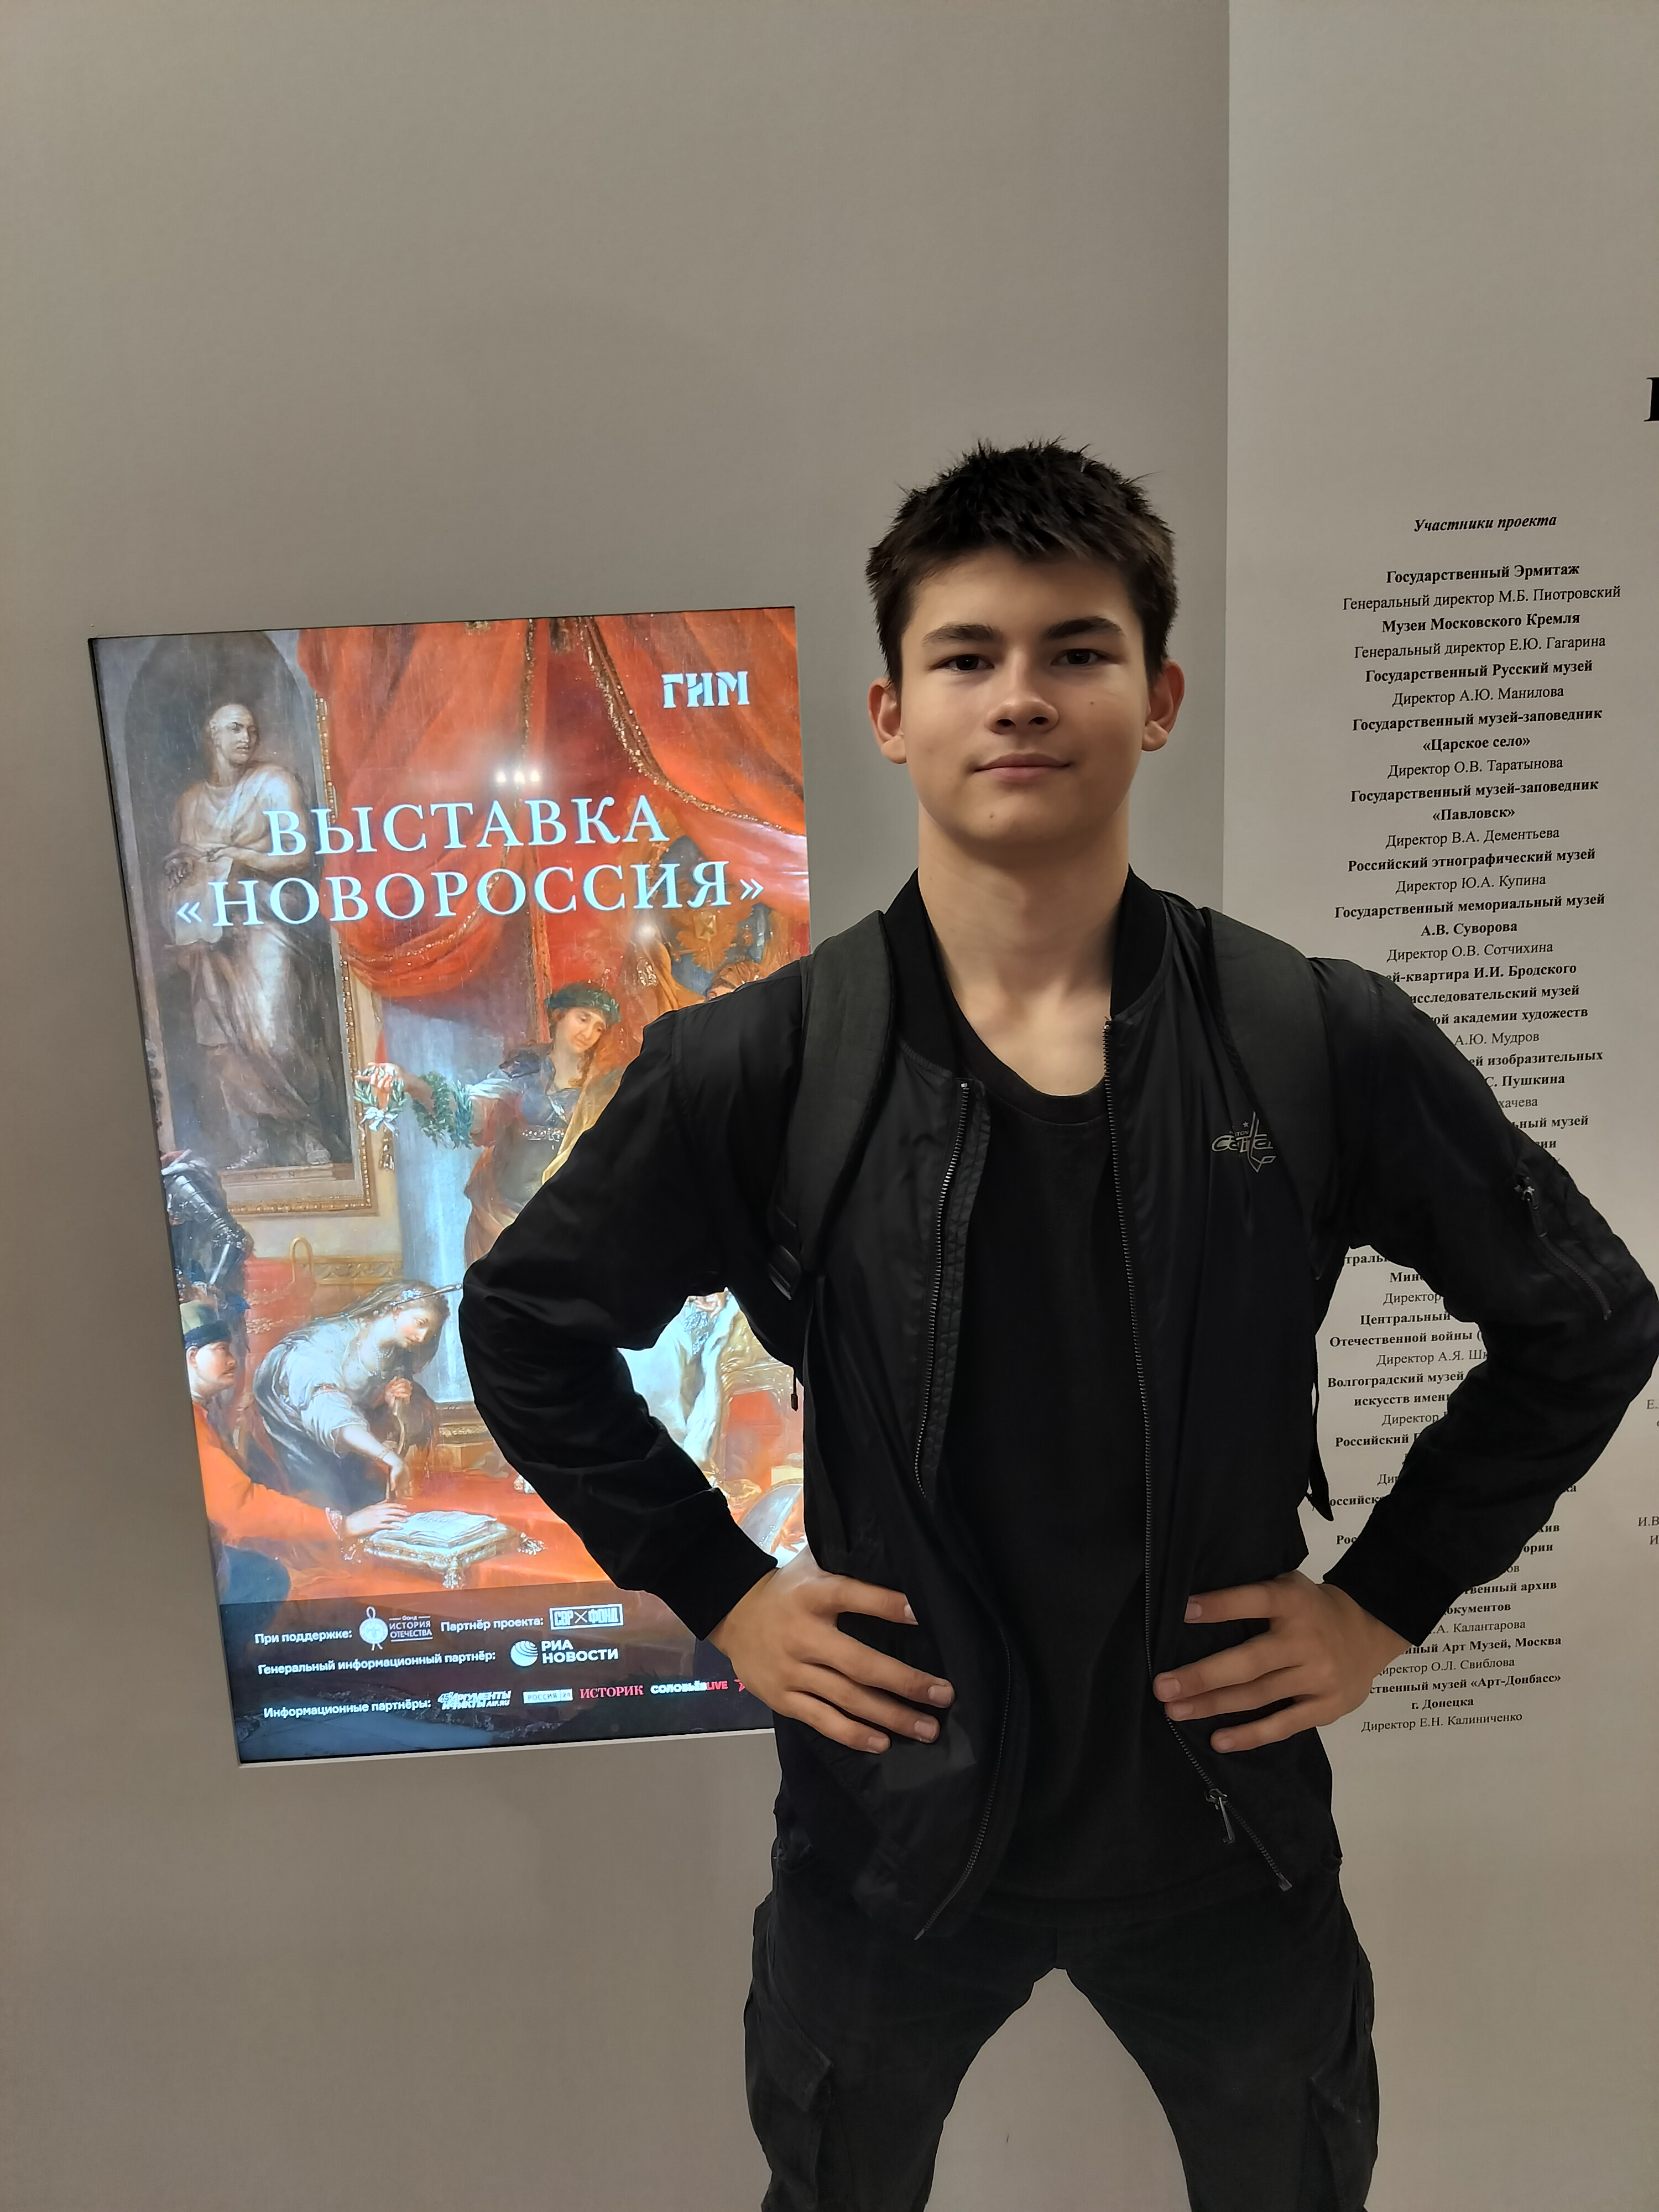
\includegraphics[width=0.4\textwidth]{images/self.jpg}
	%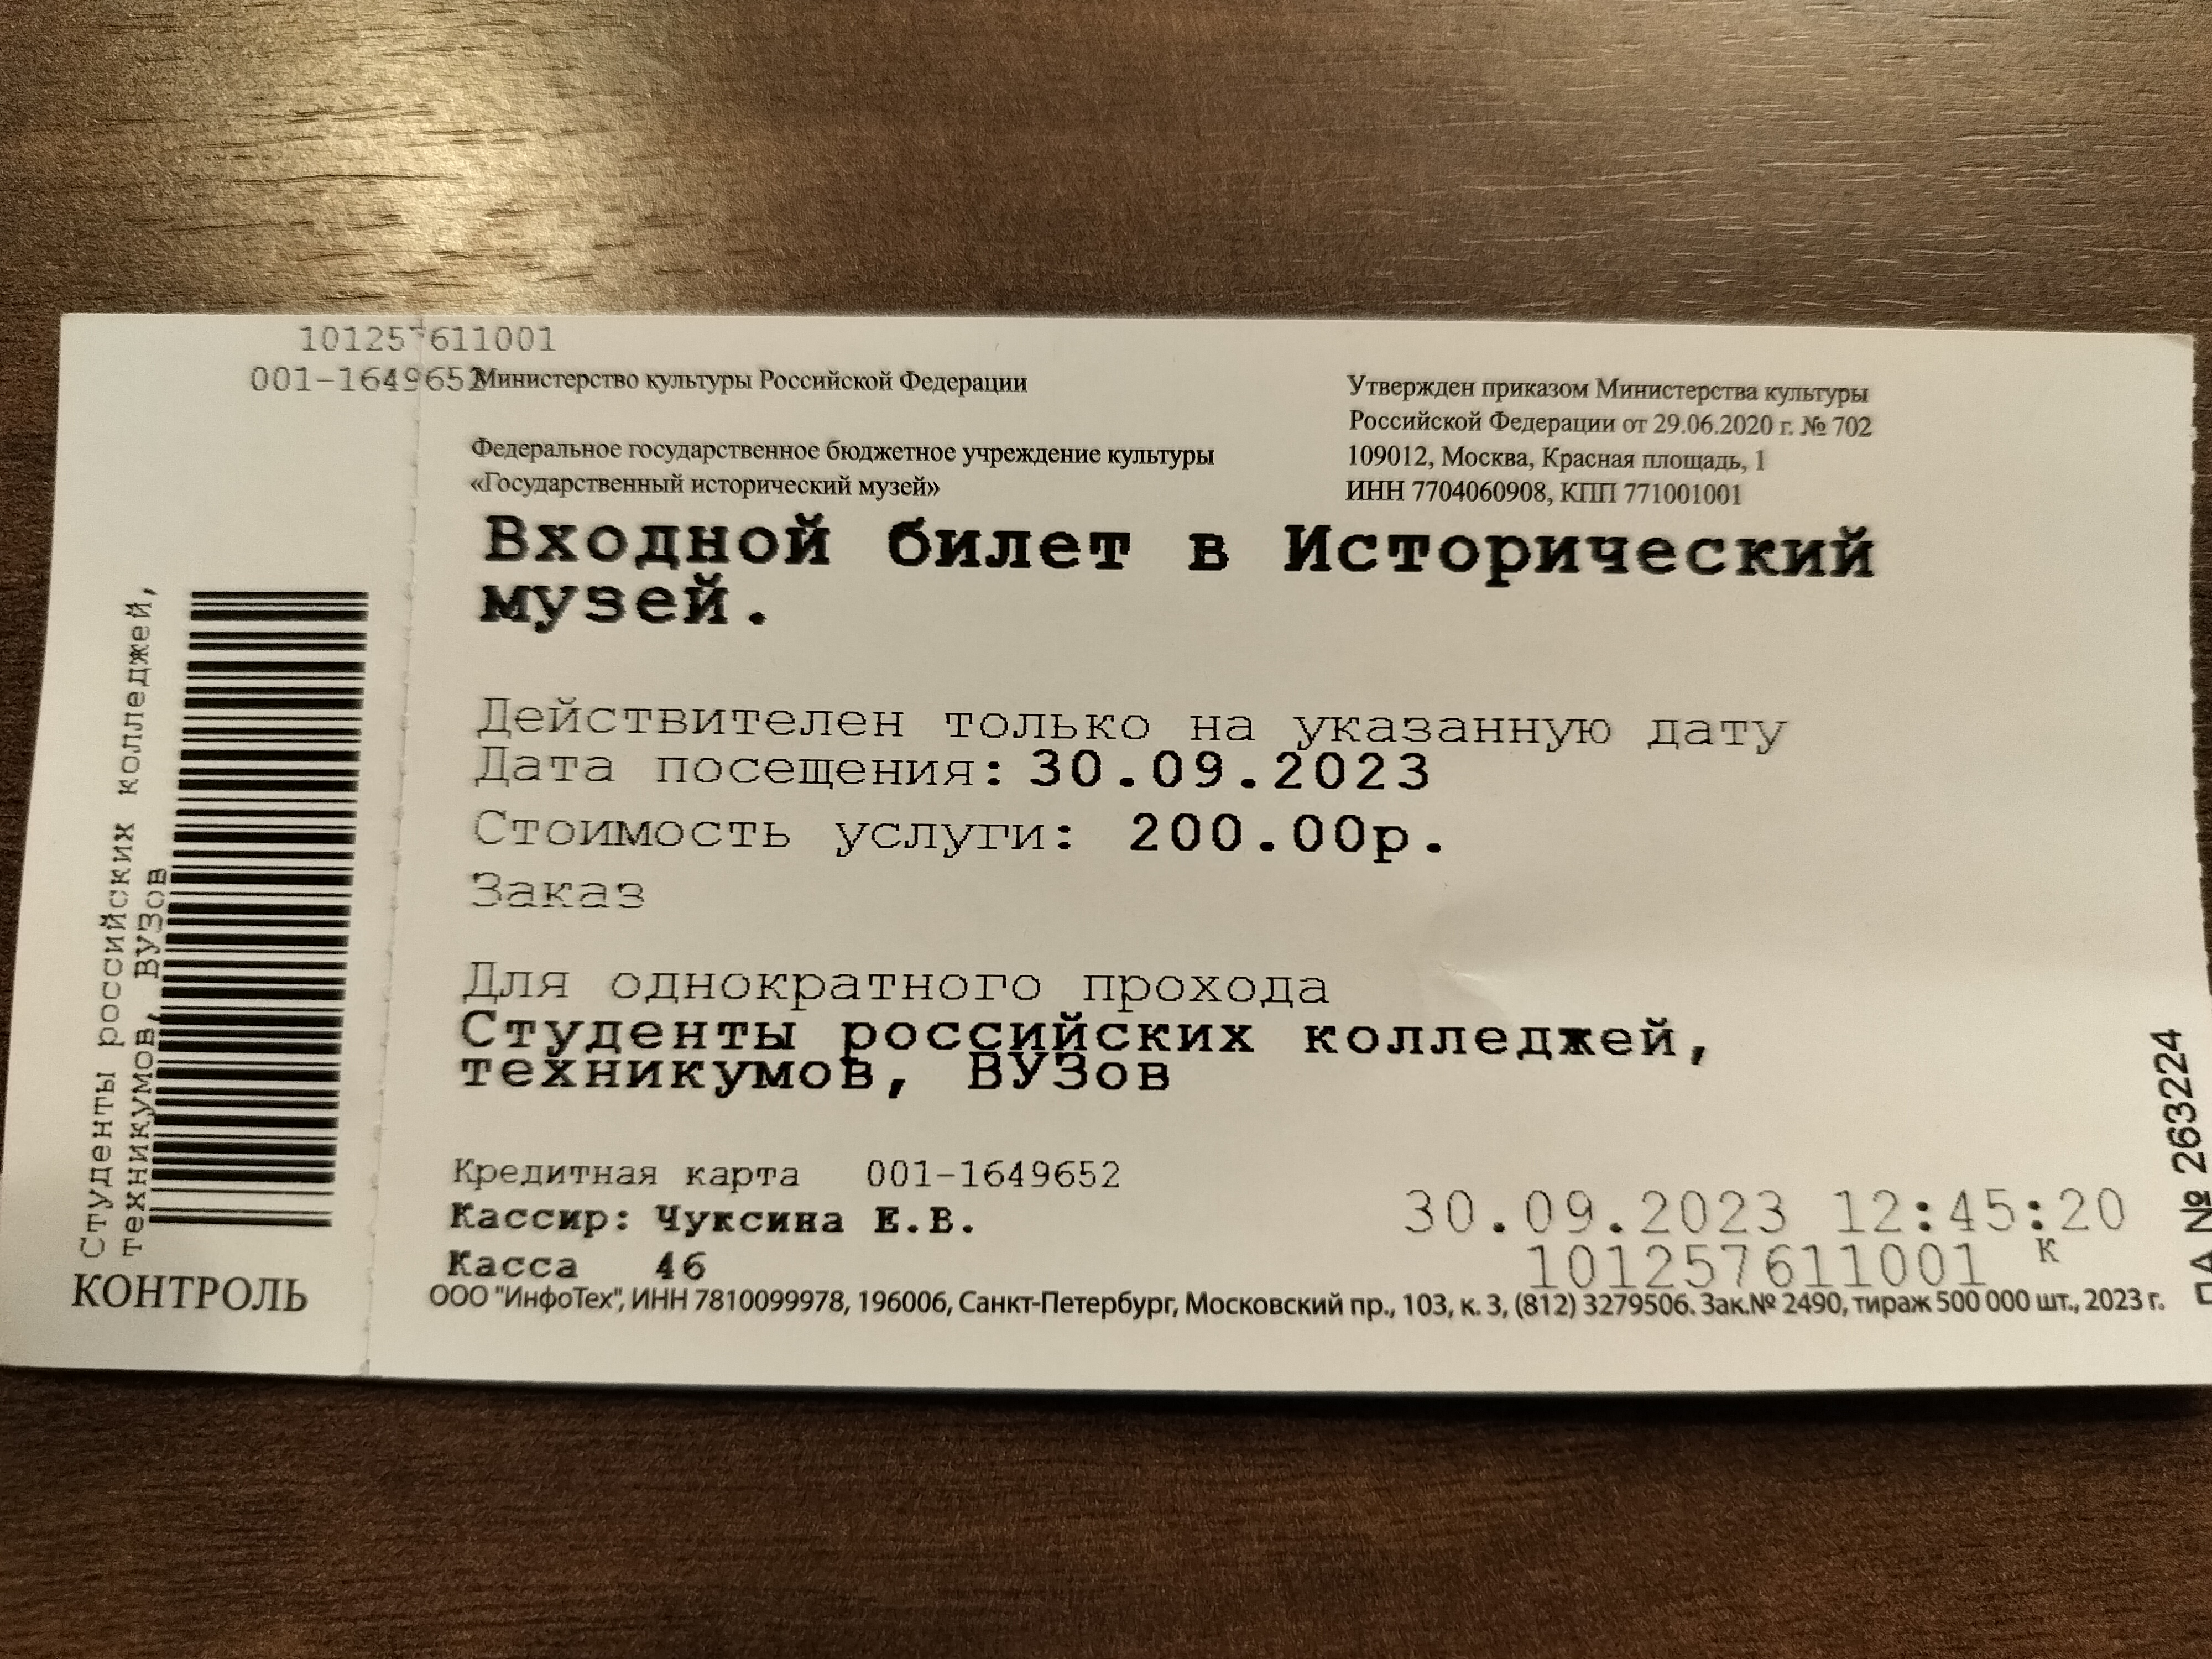
\includegraphics[width=0.4\textwidth]{images/ticket.jpg}
	Краткая история гражданской войны (1962г) Г.Г.Алахвердов, Н.Ф.Кузьмин
	\url{}
	\url{}
\end{frame}



\section{Благоданость}
\begin{frame}
	\centering
	\huge
	Спасибо за внимание!
\end{frame}


\end{document}
